% Created by tikzDevice version 0.12.3.1 on 2021-08-05 01:46:44
% !TEX encoding = UTF-8 Unicode
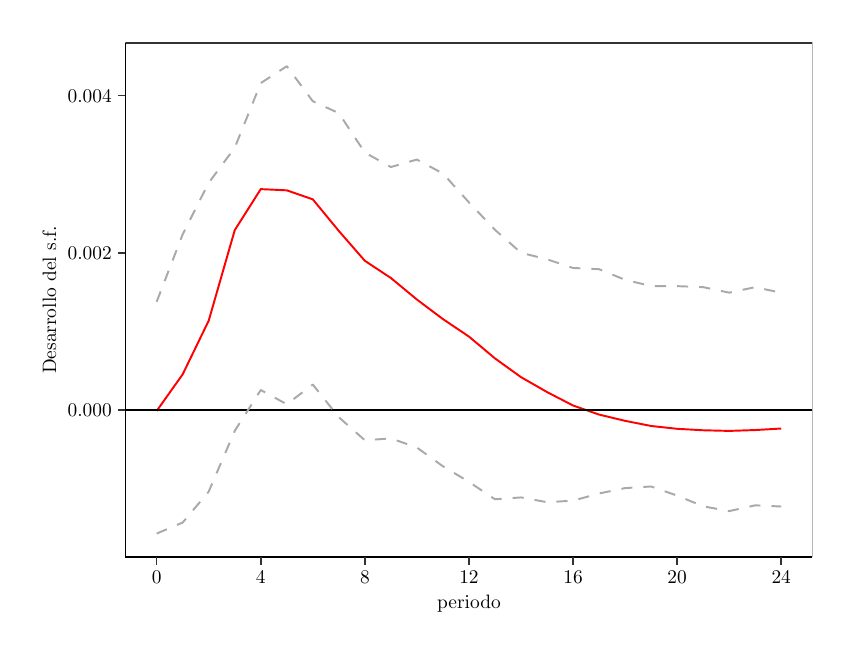
\begin{tikzpicture}[x=1pt,y=1pt]
\definecolor{fillColor}{RGB}{255,255,255}
\path[use as bounding box,fill=fillColor,fill opacity=0.00] (0,0) rectangle (289.08,216.81);
\begin{scope}
\path[clip] (  0.00,  0.00) rectangle (289.08,216.81);
\definecolor{drawColor}{RGB}{255,255,255}
\definecolor{fillColor}{RGB}{255,255,255}

\path[draw=drawColor,line width= 0.6pt,line join=round,line cap=round,fill=fillColor] (  0.00,  0.00) rectangle (289.08,216.81);
\end{scope}
\begin{scope}
\path[clip] ( 35.32, 25.56) rectangle (283.58,211.31);
\definecolor{drawColor}{RGB}{255,0,0}

\path[draw=drawColor,line width= 0.7pt,line join=round] ( 46.61, 78.31) --
	( 56.01, 91.55) --
	( 65.41,110.92) --
	( 74.82,143.63) --
	( 84.22,158.47) --
	( 93.63,158.03) --
	(103.03,154.77) --
	(112.43,143.36) --
	(121.84,132.56) --
	(131.24,126.36) --
	(140.64,118.58) --
	(150.05,111.51) --
	(159.45,105.19) --
	(168.85, 97.31) --
	(178.26, 90.53) --
	(187.66, 85.14) --
	(197.07, 80.28) --
	(206.47, 77.00) --
	(215.87, 74.74) --
	(225.28, 72.88) --
	(234.68, 71.86) --
	(244.08, 71.33) --
	(253.49, 71.10) --
	(262.89, 71.41) --
	(272.30, 71.96);
\definecolor{drawColor}{RGB}{0,0,0}

\path[draw=drawColor,line width= 0.6pt,line join=round] ( 35.32, 78.62) -- (283.58, 78.62);
\definecolor{drawColor}{RGB}{169,169,169}

\path[draw=drawColor,line width= 0.7pt,dash pattern=on 4pt off 4pt ,line join=round] ( 46.61,117.77) --
	( 56.01,142.13) --
	( 65.41,160.75) --
	( 74.82,173.41) --
	( 84.22,196.78) --
	( 93.63,202.87) --
	(103.03,190.23) --
	(112.43,185.92) --
	(121.84,171.67) --
	(131.24,166.45) --
	(140.64,169.15) --
	(150.05,164.12) --
	(159.45,153.68) --
	(168.85,143.76) --
	(178.26,135.47) --
	(187.66,133.11) --
	(197.07,129.98) --
	(206.47,129.53) --
	(215.87,125.70) --
	(225.28,123.45) --
	(234.68,123.41) --
	(244.08,123.05) --
	(253.49,121.06) --
	(262.89,123.04) --
	(272.30,121.01);

\path[draw=drawColor,line width= 0.7pt,dash pattern=on 4pt off 4pt ,line join=round] ( 46.61, 34.01) --
	( 56.01, 37.99) --
	( 65.41, 49.15) --
	( 74.82, 71.09) --
	( 84.22, 85.87) --
	( 93.63, 80.74) --
	(103.03, 87.84) --
	(112.43, 76.05) --
	(121.84, 67.71) --
	(131.24, 68.40) --
	(140.64, 65.09) --
	(150.05, 58.32) --
	(159.45, 52.68) --
	(168.85, 46.40) --
	(178.26, 47.06) --
	(187.66, 45.34) --
	(197.07, 45.89) --
	(206.47, 48.49) --
	(215.87, 50.43) --
	(225.28, 51.02) --
	(234.68, 47.72) --
	(244.08, 43.85) --
	(253.49, 42.12) --
	(262.89, 44.21) --
	(272.30, 43.78);
\definecolor{drawColor}{gray}{0.20}

\path[draw=drawColor,line width= 0.6pt,line join=round,line cap=round] ( 35.32, 25.56) rectangle (283.58,211.31);
\end{scope}
\begin{scope}
\path[clip] (  0.00,  0.00) rectangle (289.08,216.81);
\definecolor{drawColor}{RGB}{0,0,0}

\path[draw=drawColor,line width= 0.6pt,line join=round] ( 35.32, 25.56) --
	( 35.32,211.31);
\end{scope}
\begin{scope}
\path[clip] (  0.00,  0.00) rectangle (289.08,216.81);
\definecolor{drawColor}{RGB}{0,0,0}

\node[text=drawColor,anchor=base east,inner sep=0pt, outer sep=0pt, scale=  0.70] at ( 30.37, 76.21) {0.000};

\node[text=drawColor,anchor=base east,inner sep=0pt, outer sep=0pt, scale=  0.70] at ( 30.37,133.04) {0.002};

\node[text=drawColor,anchor=base east,inner sep=0pt, outer sep=0pt, scale=  0.70] at ( 30.37,189.86) {0.004};
\end{scope}
\begin{scope}
\path[clip] (  0.00,  0.00) rectangle (289.08,216.81);
\definecolor{drawColor}{gray}{0.20}

\path[draw=drawColor,line width= 0.6pt,line join=round] ( 32.57, 78.62) --
	( 35.32, 78.62);

\path[draw=drawColor,line width= 0.6pt,line join=round] ( 32.57,135.45) --
	( 35.32,135.45);

\path[draw=drawColor,line width= 0.6pt,line join=round] ( 32.57,192.27) --
	( 35.32,192.27);
\end{scope}
\begin{scope}
\path[clip] (  0.00,  0.00) rectangle (289.08,216.81);
\definecolor{drawColor}{RGB}{0,0,0}

\path[draw=drawColor,line width= 0.6pt,line join=round] ( 35.32, 25.56) --
	(283.58, 25.56);
\end{scope}
\begin{scope}
\path[clip] (  0.00,  0.00) rectangle (289.08,216.81);
\definecolor{drawColor}{gray}{0.20}

\path[draw=drawColor,line width= 0.6pt,line join=round] ( 46.61, 22.81) --
	( 46.61, 25.56);

\path[draw=drawColor,line width= 0.6pt,line join=round] ( 84.22, 22.81) --
	( 84.22, 25.56);

\path[draw=drawColor,line width= 0.6pt,line join=round] (121.84, 22.81) --
	(121.84, 25.56);

\path[draw=drawColor,line width= 0.6pt,line join=round] (159.45, 22.81) --
	(159.45, 25.56);

\path[draw=drawColor,line width= 0.6pt,line join=round] (197.07, 22.81) --
	(197.07, 25.56);

\path[draw=drawColor,line width= 0.6pt,line join=round] (234.68, 22.81) --
	(234.68, 25.56);

\path[draw=drawColor,line width= 0.6pt,line join=round] (272.30, 22.81) --
	(272.30, 25.56);
\end{scope}
\begin{scope}
\path[clip] (  0.00,  0.00) rectangle (289.08,216.81);
\definecolor{drawColor}{RGB}{0,0,0}

\node[text=drawColor,anchor=base,inner sep=0pt, outer sep=0pt, scale=  0.70] at ( 46.61, 15.79) {0};

\node[text=drawColor,anchor=base,inner sep=0pt, outer sep=0pt, scale=  0.70] at ( 84.22, 15.79) {4};

\node[text=drawColor,anchor=base,inner sep=0pt, outer sep=0pt, scale=  0.70] at (121.84, 15.79) {8};

\node[text=drawColor,anchor=base,inner sep=0pt, outer sep=0pt, scale=  0.70] at (159.45, 15.79) {12};

\node[text=drawColor,anchor=base,inner sep=0pt, outer sep=0pt, scale=  0.70] at (197.07, 15.79) {16};

\node[text=drawColor,anchor=base,inner sep=0pt, outer sep=0pt, scale=  0.70] at (234.68, 15.79) {20};

\node[text=drawColor,anchor=base,inner sep=0pt, outer sep=0pt, scale=  0.70] at (272.30, 15.79) {24};
\end{scope}
\begin{scope}
\path[clip] (  0.00,  0.00) rectangle (289.08,216.81);
\definecolor{drawColor}{RGB}{0,0,0}

\node[text=drawColor,anchor=base,inner sep=0pt, outer sep=0pt, scale=  0.70] at (159.45,  6.86) {periodo};
\end{scope}
\begin{scope}
\path[clip] (  0.00,  0.00) rectangle (289.08,216.81);
\definecolor{drawColor}{RGB}{0,0,0}

\node[text=drawColor,rotate= 90.00,anchor=base,inner sep=0pt, outer sep=0pt, scale=  0.70] at ( 10.32,118.44) {Desarrollo del s.f.};
\end{scope}
\end{tikzpicture}
